\chapter{Kesetimbangan Redoks dan Persamaan Nernst}\label{ch:b1:nernst}

Masukkan sekeping seng ke dalam larutan seng sulfat, sekeping tembaga ke
dalam larutan tembaga(II) sulfat, hubungkan kedua larutan dengan sebuah
tabung berisi larutan garam dan kedua logam dengan kawat melalui sebuah
dioda pemancar cahaya: diodanya menyala. Reaksi seng dengan ion tembaga,
yang di dalam satu gelas kimia hanya menghangatkan larutan, kini
mendorong elektron melalui kawat. Sebuah baterai adalah susunan ini dalam
kemasan; pH meter dan elektrode klorida adalah sepupu pengukurnya. Bab
ini menyatakan pertukaran elektron itu dengan angka: \omterm{def:b1:nernst:oxidation-number}{bilangan oksidasi}
untuk menghitung elektron, \omterm{def:b1:nernst:electrode-potential}{potensial elektrode} untuk mengurutkan
pasangan-pasangan, dan \omterm{thm:b1:nernst:nernst}{persamaan Nernst} untuk mengikutinya terhadap
konsentrasi.

\begin{recall}
Jilid sekolah (kelas 11 dan 12) mendefinisikan \omterm{def:b1:nernst:couple}{oksidator} dan \omterm{def:b1:nernst:couple}{reduktor},
menuliskan \omterm{def:b1:nernst:couple}{setengah reaksi}, menyusun sel dari dua logam dan dua larutan,
dan membaca sel seng--tembaga sebagai sebuah baterai. \omterm{def:b1:extent-q-and-k:quotient}{Kuosien reaksi} dan
tetapan kesetimbangan adalah yang pada \cref{ch:b1:extent-q-and-k};
\omterm{def:b1:extent-q-and-k:activity}{aktivitasnya} $c/c^\circ$ untuk zat terlarut dan $p/p^\circ$ untuk gas,
1 untuk padatan dan zat cair murni.
\end{recall}

\section{Bilangan oksidasi dan pasangan redoks}

\begin{definition}[Oksidator, reduktor, pasangan redoks, setengah reaksi]\label{def:b1:nernst:couple}
\emph{Oksidator}\index{oksidator} adalah spesies yang mampu menerima
elektron, \emph{reduktor}\index{reduktor} spesies yang mampu
memberikannya. Oksidator Ox dan reduktor Red yang terbentuk darinya
membentuk sebuah \emph{pasangan redoks}\index{pasangan redoks} Ox/Red,
yang dipaparkan oleh \emph{setengah reaksi}\index{setengah reaksi} pasangan itu,
$\alpha\,\mathrm{Ox} + n\,\mathrm{e^-} \rightleftharpoons
\beta\,\mathrm{Red}$, yang disetarakan atomnya dengan \ce{H2O} dan
\ce{H+} bila perlu dan muatannya dengan elektron.
\end{definition}

Reaksi redoks adalah pertukaran elektron antara dua pasangan: \omterm{def:b1:nernst:couple}{oksidator}
pasangan yang satu tereduksi sementara \omterm{def:b1:nernst:couple}{reduktor} pasangan yang lain
teroksidasi, dan elektron-elektronnya saling meniadakan. Untuk
menghitungnya dalam spesies yang rumit, setiap atom diberi \omterm{def:b1:nernst:oxidation-number}{bilangan
oksidasi}.

\begin{definition}[Bilangan oksidasi]\label{def:b1:nernst:oxidation-number}
\emph{Bilangan oksidasi}\index{bilangan oksidasi} sebuah atom dalam suatu
spesies adalah muatan yang akan dibawanya seandainya setiap ikatan
diputus dengan memberikan kedua elektron ikatan kepada atom yang lebih
elektronegatif (dibagi sama rata antara dua atom yang identik). Bilangan
ini ditulis dengan angka Romawi: besi(III), \ce{Mn^{+VII}} dalam ion
permanganat.
\end{definition}

\begin{proposition}[Aturan bilangan oksidasi]\label{prop:b1:nernst:on-rules}
\begin{enumerate}
  \item Atom dalam unsur bebas mempunyai \omterm{def:b1:nernst:oxidation-number}{bilangan oksidasi} 0; ion
        monoatomik mempunyai \omterm{def:b1:nernst:oxidation-number}{bilangan oksidasi} sama dengan muatannya.
  \item Jumlah \omterm{def:b1:nernst:oxidation-number}{bilangan oksidasi} atom-atom sebuah spesies sama dengan
        muatannya.
  \item Hidrogen $+$I (kecuali dalam hidrida logam, $-$I); oksigen
        $-$II (kecuali dalam peroksida, $-$I, dan jika terikat pada
        fluorin); fluorin $-$I.
  \item Dalam \omterm{def:b1:nernst:couple}{setengah reaksi}, banyaknya elektron sama dengan perubahan
        \omterm{def:b1:nernst:oxidation-number}{bilangan oksidasi} unsur yang berubah dikalikan dengan banyaknya
        atom unsur itu.
\end{enumerate}
\end{proposition}

\begin{proof}
1 dan 2: memutus semua ikatan mempertahankan muatan, dan antara atom-atom
yang identik tidak ada yang dipindahkan. 3: hidrogen kurang elektronegatif
daripada setiap nonlogam yang berikatan dengannya (\cref{ch:b1:periodicity})
dan lebih elektronegatif daripada logam alkali; oksigen lebih
elektronegatif daripada setiap unsur kecuali fluorin, dan dalam \ce{O-O}
pasangan bersamanya dibagi dua. 4: H dan O mempertahankan bilangannya,
sehingga satu-satunya atom yang muatan fiktifnya berubah adalah atom
unsur yang bersangkutan, dan elektron muncul dalam \omterm{def:b1:nernst:couple}{setengah reaksi} tepat
untuk menyetarakan perubahan muatan itu.
\end{proof}

\begin{method}[Bilangan oksidasi sebuah spesies]\label{met:b1:nernst:oxidation-numbers}
Berikan bilangan yang biasa kepada H, O, F, dan ion-ion; bilangan atom
yang tersisa diperoleh dari aturan 2. Dalam \ce{MnO4-}: $x + 4(-2) = -1$,
$x = +7$. Dalam \ce{Cr2O7^2-}: $2x - 14 = -2$, $x = +6$. Dalam
\ce{S4O6^2-}, rata-ratanya $+2.5$; \omterm{def:b1:lewis-resonance-vsepr:lewis}{struktur Lewis} memperlihatkan dua jenis
belerang.
\end{method}

\begin{method}[Menyetarakan setengah reaksi]\label{met:b1:nernst:balance-by-on}
\begin{enumerate}
  \item Setarakan unsur yang berubah \omterm{def:b1:nernst:oxidation-number}{bilangan oksidasinya}.
  \item Tambahkan elektron: perubahan \omterm{def:b1:nernst:oxidation-number}{bilangan oksidasi} dikalikan dengan
        banyaknya atom.
  \item Setarakan muatan dengan \ce{H+} (larutan asam) atau \ce{OH-}
        (larutan basa).
  \item Setarakan hidrogen dan oksigen dengan \ce{H2O}; periksalah
        oksigen paling akhir.
\end{enumerate}
Untuk ion permanganat dalam asam: Mn berubah dari $+$VII ke $+$II,
sehingga 5 elektron; muatan di ruas kiri $-1 - 5 = -6$ dan di ruas kanan
$+2$, sehingga $8\,\ce{H+}$; lalu $4\,\ce{H2O}$:
\ce{MnO4- + 8H+ + 5e- -> Mn^2+ + 4H2O}.
\end{method}

\section{Sel elektrokimia}

\begin{definition}[Sel elektrokimia]\label{def:b1:nernst:cell}
\emph{Sel elektrokimia}\index{sel elektrokimia} terdiri atas dua
\emph{setengah sel}\index{setengah sel}, masing-masing tersusun atas
sebuah \omterm{def:b1:nernst:couple}{pasangan redoks} dan sebuah konduktor elektronik, yaitu elektrode,
yang dihubungkan oleh konduktor ionik, sering kali sebuah \emph{jembatan
garam}\index{jembatan garam} (gel atau tabung berisi garam inert yang
pekat seperti kalium nitrat). Elektrode tempat oksidasi berlangsung
adalah \emph{anode}\index{anode}, elektrode tempat reduksi berlangsung
adalah \emph{katode}\index{katode}.
\emph{Tegangan sel}\index{tegangan sel} adalah beda potensial listrik antara kedua elektrode, kutub positif
dikurangi kutub negatif, yang diukur ketika tidak ada arus yang
mengalir.
\end{definition}

\begin{omfigure}
\begin{tikzpicture}[font=\small, >={Stealth}]
  \pic at (0,0) {beaker={0.7}{omDef!14}};
  \pic at (3.6,0) {beaker={0.7}{omDef!32}};
  \pic at (-0.3,0.25) {electrode={black!35}};
  \pic at (3.9,0.25) {electrode={orange!70!brown}};
  \pic at (0.35,0.55) {saltbridge={2.9}};
  \pic (m) at (1.8,4.3) {meter={V}};
  \draw[thick] (-0.15,2.65) |- (m-a);
  \draw[thick] (4.05,2.65) |- (m-b);
  \node[anchor=east] at (-0.95,1.0) {\ce{Zn}};
  \node[anchor=west] at (4.45,1.0) {\ce{Cu}};
  \node at (0.25,-0.35) {\ce{Zn^2+}, \ce{SO4^2-}};
  \node at (3.6,-0.35) {\ce{Cu^2+}, \ce{SO4^2-}};
  \draw[->, omProp, thick] (-0.15,3.35) -- (0.8,3.35) node[above, midway] {$\mathrm{e^-}$};
  \draw[->, omProp, thick] (2.8,3.35) -- (3.75,3.35) node[above, midway] {$\mathrm{e^-}$};
  \node[anchor=east] at (-0.9,2.3) {$-$ anode};
  \node[anchor=west] at (4.6,2.3) {katode $+$};
  \node[font=\scriptsize, align=center] at (1.8,2.75) {jembatan garam\\ \ce{K+} $\rightarrow$ \quad $\leftarrow$ \ce{NO3-}};
  \node[font=\scriptsize] at (-0.1,-0.8) {\ce{Zn -> Zn^2+ + 2e-}};
  \node[font=\scriptsize] at (3.7,-0.8) {\ce{Cu^2+ + 2e- -> Cu}};
\end{tikzpicture}

{\small Sel seng--tembaga (sel Daniell). Seng teroksidasi di \omterm{def:b1:nernst:cell}{anode}, kutub
negatif; ion-ion tembaga tereduksi di \omterm{def:b1:nernst:cell}{katode}, kutub positif. Elektron
mengalir melalui rangkaian luar dari seng ke tembaga; di dalam \omterm{def:b1:nernst:cell}{jembatan
garam} kation-kation bergerak ke \omterm{def:b1:nernst:cell}{katode} dan anion-anion ke \omterm{def:b1:nernst:cell}{anode}, sehingga
setiap larutan tetap netral.}
\end{omfigure}

Sebuah sel ditulis sebagai satu baris, dengan \omterm{def:b1:nernst:cell}{anode} di kiri: \ce{Zn} $|$
\ce{Zn^2+} $\|$ \ce{Cu^2+} $|$ \ce{Cu}, garis tunggal untuk antarmuka,
garis ganda untuk \omterm{def:b1:nernst:cell}{jembatan garam}. Jika semua konsentrasi
\qty{1}{mol/L}, tegangannya \qty{1.10}{V}. Reaksi yang berlangsung ketika
sel mengalirkan arus, \ce{Zn + Cu^2+ -> Zn^2+ + Cu}, adalah reaksi yang
akan terjadi di dalam satu gelas kimia; memisahkan kedua \omterm{def:b1:nernst:cell}{setengah sel}
memaksa elektron melewati kawat, tempat elektron itu dapat melakukan
usaha.

\section{Potensial elektrode}

Tegangan adalah sebuah selisih: hanya selisih antara dua \omterm{def:b1:nernst:cell}{setengah sel}
yang dapat diukur. Karena itu dipilih satu \omterm{def:b1:nernst:cell}{setengah sel} acuan untuk
selamanya.

\begin{definition}[Potensial elektrode, potensial standar]\label{def:b1:nernst:electrode-potential}
\emph{Elektrode hidrogen standar}\index{elektrode hidrogen standar} adalah
elektrode platina yang bersentuhan dengan gas hidrogen pada \qty{1}{bar}
dan larutan ideal \ce{H+} beraktivitas 1. \emph{Potensial
elektrode}\index{potensial elektrode} $E$ sebuah \omterm{def:b1:nernst:cell}{setengah sel} adalah
\omterm{def:b1:nernst:cell}{tegangan sel} yang dibentuk dengan elektrode hidrogen standar di sebelah
kiri: $E = V_{\text{setengah sel}} - V_{\text{EHS}}$. Jika setiap spesies
pasangan itu beraktivitas 1, potensial itu adalah \emph{potensial
standar}\index{potensial standar} $E^\circ$ pasangan itu, sebuah tetapan
pada suhu tertentu.
\end{definition}

\begin{omfigure}
\begin{tikzpicture}[font=\small, >={Stealth}]
  \pic at (0,0) {beaker={0.72}{omDef!14}};
  % glass jacket, open at the bottom, with the gas inlet on the right
  \draw[om glass] (-0.32,0.35) -- (-0.32,3.0) -- (0.32,3.0) -- (0.32,2.55)
    -- (0.95,2.55) (0.32,2.35) -- (0.95,2.35) (0.32,2.35) -- (0.32,0.35);
  \draw[thick] (0,0.9) -- (0,3.45);
  \fill[black!60] (-0.16,0.5) rectangle (0.16,0.9);
  \foreach \x/\y in {0.45/0.45, 0.55/0.75, 0.48/1.05, -0.45/0.5, -0.52/0.85}
    \draw[omDef!70] (\x,\y) circle (0.055);
  \draw[->] (1.9,2.45) node[right] {\ce{H2}, \qty{1}{bar}} -- (1.0,2.45);
  \draw (0.12,0.7) -- (1.5,0.2) node[right] {platina terplatinasi};
  \draw (-0.6,1.1) -- (-1.4,1.6) node[left] {\ce{H+}, aktivitas 1};
  \node[anchor=west] at (0.05,3.45) {ke rangkaian};
\end{tikzpicture}

{\small \omterm{def:b1:nernst:electrode-potential}{Elektrode hidrogen standar}: gas hidrogen digelembungkan di atas
pelat platina yang dilapisi platina halus, yang dicelupkan ke dalam
larutan dengan \omterm{def:b1:extent-q-and-k:activity}{aktivitas} \ce{H+} sama dengan 1. Pasangannya adalah
\ce{H+}/\ce{H2}, dengan potensial 0 menurut konvensi.}
\end{omfigure}

Elektrode hidrogen sulit dipakai; laboratorium mengukur terhadap \omterm{def:b1:nernst:cell}{setengah
sel} yang lebih praktis yang potensialnya diketahui.

\begin{definition}[Elektrode acuan]\label{def:b1:nernst:reference-electrode}
\emph{Elektrode acuan}\index{elektrode acuan} adalah \omterm{def:b1:nernst:cell}{setengah sel} yang
potensialnya tetap dan diketahui: elektrode perak--perak klorida (kawat
perak yang dilapisi perak klorida dalam larutan klorida berkonsentrasi
tetap) atau elektrode kalomel (raksa yang bersentuhan dengan
\ce{Hg2Cl2} dan larutan klorida).
\end{definition}

Tabel di bawah memberikan \omterm{def:b1:nernst:electrode-potential}{potensial standar} yang dipakai dalam jilid ini;
skala vertikal pada subbab berikutnya memperlihatkan yang paling umum.

\begin{omfigure}
\begin{tabular}{lr@{\qquad}lr}
\hline
pasangan & $E^\circ$ (V) & pasangan & $E^\circ$ (V) \\
\hline
\ce{Li+}/\ce{Li} & $-3.04$ & \ce{Cu^2+}/\ce{Cu} & 0.34 \\
\ce{K+}/\ce{K} & $-2.94$ & $[\ce{Fe(CN)6}]^{3-}$/$[\ce{Fe(CN)6}]^{4-}$ & 0.36 \\
\ce{Na+}/\ce{Na} & $-2.71$ & \ce{Cu+}/\ce{Cu} & 0.52 \\
\ce{Mg^2+}/\ce{Mg} & $-2.36$ & \ce{I2}/\ce{I-} & 0.53 \\
\ce{Al^3+}/\ce{Al} & $-1.68$ & \ce{O2}/\ce{H2O2} & 0.69 \\
\ce{Zn^2+}/\ce{Zn} & $-0.76$ & \ce{Fe^3+}/\ce{Fe^2+} & 0.77 \\
\ce{Fe^2+}/\ce{Fe} & $-0.41$ & \ce{Hg2^2+}/\ce{Hg} & 0.80 \\
\ce{Ni^2+}/\ce{Ni} & $-0.24$ & \ce{Ag+}/\ce{Ag} & 0.80 \\
\ce{Pb^2+}/\ce{Pb} & $-0.13$ & \ce{Br2}/\ce{Br-} & 1.08 \\
\ce{H+}/\ce{H2} & 0 & \ce{O2}/\ce{H2O} & 1.23 \\
\ce{S4O6^2-}/\ce{S2O3^2-} & 0.02 & \ce{MnO2}/\ce{Mn^2+} & 1.23 \\
\ce{Cu^2+}/\ce{Cu+} & 0.16 & \ce{Cl2}/\ce{Cl-} & 1.36 \\
\ce{AgCl}/\ce{Ag} & 0.22 & \ce{PbO2}/\ce{Pb^2+} & 1.46 \\
\ce{Hg2Cl2}/\ce{Hg} & 0.27 & \ce{MnO4-}/\ce{Mn^2+} & 1.51 \\
 & & \ce{HClO}/\ce{Cl2} & 1.63 \\
 & & \ce{H2O2}/\ce{H2O} & 1.76 \\
\hline
\end{tabular}

\smallskip
{\small \omterm{def:b1:nernst:electrode-potential}{Potensial standar} pada \qty{25}{\celsius}, yang dihitung dari
energi Gibbs pembentukan standar spesies-spesies setiap pasangan dalam
tabel. Nilainya dapat berbeda beberapa perseratus volt dari kompilasi
lain.}
% ledger: dfg:Li+_ao, dfg:K+_ao, dfg:Na+_ao, dfg:Mg2+_ao, dfg:Al3+_ao, dfg:Zn2+_ao, dfg:Fe2+_ao, dfg:Ni2+_ao, dfg:Pb2+_ao (computed in figdata/bachelor-1/standard-potentials.py)
% ledger: dfg:S4O62-_ao, dfg:S2O32-_ao, dfg:Cu2+_ao, dfg:Cu+_ao, dfg:AgCl_cr, dfg:Cl-_ao, dfg:Hg2Cl2_cr, dfg:Fe_CN63-_ao, dfg:Fe_CN64-_ao, dfg:I-_ao (same script)
% ledger: dfg:H2O2_ao, dfg:Fe3+_ao, dfg:Hg22+_ao, dfg:Ag+_ao, dfg:Br-_ao, dfg:H2O_l, dfg:MnO2_cr, dfg:Mn2+_ao, dfg:PbO2_cr, dfg:MnO4-_ao, dfg:HClO_ao (same script)
\end{omfigure}

\section{Persamaan Nernst}

\begin{theorem}[Persamaan Nernst]\label{thm:b1:nernst:nernst}
Untuk pasangan $\alpha\,\mathrm{Ox} + n\,\mathrm{e^-} \rightleftharpoons
\beta\,\mathrm{Red}$, dengan kemungkinan adanya spesies lain (\ce{H+},
\ce{H2O}, \ce{Cl-}) di salah satu ruas, \omterm{def:b1:nernst:electrode-potential}{potensial elektrodenya} diberikan
oleh \emph{persamaan Nernst}\index{persamaan Nernst}
\[
  E = E^\circ + \frac{RT}{nF}\ln\frac{\prod a_{\text{ruas oksidator}}^{\nu}}{\prod
  a_{\text{ruas reduktor}}^{\nu}}
  = E^\circ + \frac{0.059}{n}\log\frac{a(\mathrm{Ox})^\alpha\,\cdots}{a(\mathrm{Red})^\beta\,\cdots}
  \quad\text{pada \qty{25}{\celsius}},
\]
dengan setiap \omterm{def:b1:extent-q-and-k:activity}{aktivitas} dipangkatkan dengan \omterm{def:b1:extent-q-and-k:extent}{bilangan stoikiometrinya} dan
faktor $RT\ln 10/F = \qty{0.059}{V}$ pada \qty{298}{K}.
\end{theorem}

\admitted{\omterm{thm:b1:nernst:nernst}{Persamaan Nernst} diturunkan dari hubungan antara energi Gibbs
sebuah reaksi dan \omterm{def:b1:nernst:cell}{tegangan sel}, yang diturunkan dalam jilid Tahun~2.}

\begin{example}[Tiga pasangan]\label{ex:b1:nernst:examples}
\ce{Cu^2+}/\ce{Cu}: $E = 0.34 + 0.030\log[\ce{Cu^2+}]$ (logam tembaga
beraktivitas 1).
\ce{Fe^3+}/\ce{Fe^2+}: $E = 0.77 + 0.059\log([\ce{Fe^3+}]/[\ce{Fe^2+}])$.
\ce{MnO4-}/\ce{Mn^2+}: $E = 1.51 + \frac{0.059}{5}\log
\frac{[\ce{MnO4-}][\ce{H+}]^8}{[\ce{Mn^2+}]}$; pada konsentrasi
permanganat dan mangan(II) yang sama, $E = 1.51 - 0.094\,\mathrm{pH}$:
daya pengoksidasi permanganat turun seiring naiknya pH.
\end{example}

Perubahan sepuluh kali lipat sebuah konsentrasi menggeser potensial
sebesar $0.059/n$ volt: beberapa puluh milivolt. Itulah sebabnya
tegangan yang diukur sampai milivolt merupakan ukuran konsentrasi yang
akurat, prinsip elektrode pH dan elektrode klorida pada soal akhir pekan.

\begin{history}[Walther Nernst]
\begin{minipage}[t]{0.22\linewidth}\vspace{0pt}
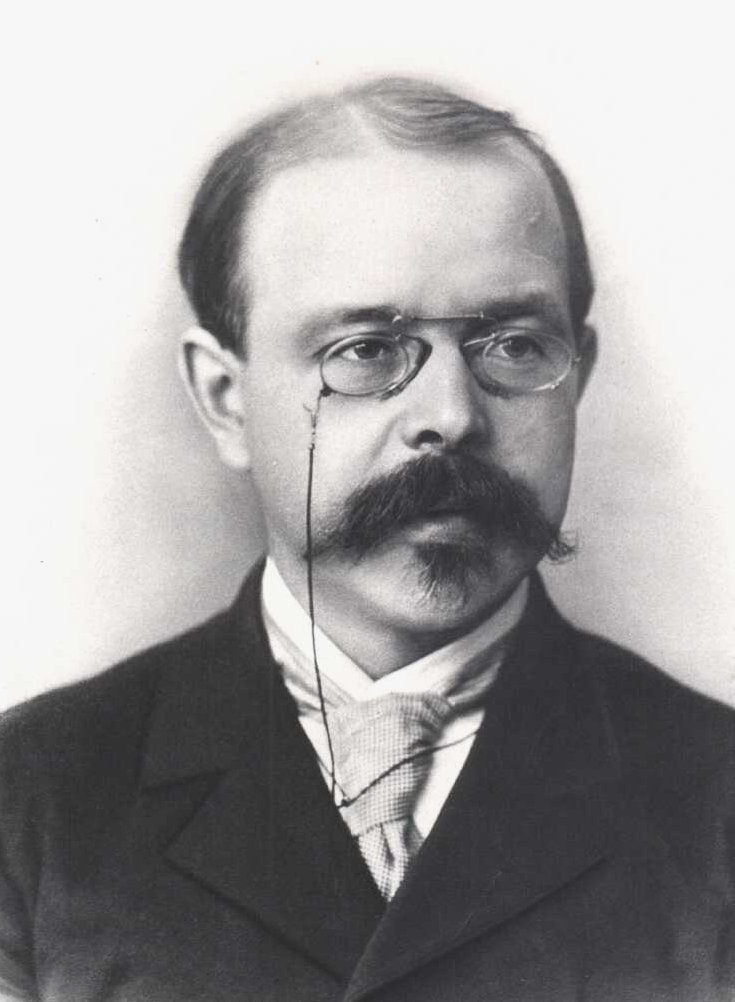
\includegraphics[width=\linewidth]{images/book2/nernst.jpg}
\end{minipage}\hfill
\begin{minipage}[t]{0.74\linewidth}\vspace{0pt}
Walther Nernst (1864--1941), di sini berusia dua puluh lima tahun, pada
1889. Persamaan dalam subbab ini, yang menghubungkan tegangan sebuah sel
dengan konsentrasi ion-ionnya, menyandang namanya, demikian pula sebuah
hukum ketiga termodinamika yang dijumpai dalam jilid Tahun~2. (Foto:
Smithsonian Libraries, domain publik, Wikimedia Commons.)
\end{minipage}
\end{history}

\section{Meramalkan reaksi redoks}

\begin{method}[Meramalkan reaksi redoks]\label{met:b1:nernst:predict-redox}
\begin{enumerate}
  \item Tempatkan pasangan-pasangan pada skala vertikal \omterm{def:b1:nernst:electrode-potential}{potensial
        standar}, \omterm{def:b1:nernst:couple}{oksidator} di kiri, \omterm{def:b1:nernst:couple}{reduktor} di kanan.
  \item \omterm{def:b1:nernst:couple}{Oksidator} terkuat yang ada ($E^\circ$ tertinggi) bereaksi dengan
        \omterm{def:b1:nernst:couple}{reduktor} terkuat yang ada ($E^\circ$ terendah): panah dari
        \omterm{def:b1:nernst:couple}{oksidator} turun ke \omterm{def:b1:nernst:couple}{reduktor}, lalu naik ke produk, membentuk huruf
        Yunani gamma, $\gamma$.
  \item Reaksi itu disukai ($K > 1$) jika pasangan \omterm{def:b1:nernst:couple}{oksidator} berada di
        atas pasangan \omterm{def:b1:nernst:couple}{reduktor}; dalam praktik reaksi itu \omterm{def:b1:extent-q-and-k:quantitative}{kuantitatif} jika
        selisihnya melebihi sekitar \qty{0.25}{V} untuk satu elektron
        yang dipertukarkan.
\end{enumerate}
\end{method}

\begin{omfigure}
\begin{tikzpicture}[font=\small, >={Stealth}, y=2.6cm]
  \draw[->, thick] (0,-1.0) -- (0,1.85) node[above] {$E^\circ$ (V)};
  \foreach \e/\o/\r in {-0.76/\ce{Zn^2+}/\ce{Zn}, 0/\ce{H+}/\ce{H2},
      0.34/\ce{Cu^2+}/\ce{Cu}, 0.77/\ce{Fe^3+}/\ce{Fe^2+},
      1.36/\ce{Cl2}/\ce{Cl-}, 1.51/\ce{MnO4-}/\ce{Mn^2+}} {
    \draw (-0.12,\e) -- (0.12,\e);
    \node[anchor=east] at (-0.25,\e) {\o};
    \node[anchor=west] at (0.25,\e) {\r};
    \node[anchor=west, black!55, font=\scriptsize] at (2.0,\e) {\e};
  }
  \node[omProp] at (-1.0,1.85) {oksidator};
  \node[omDef] at (1.1,1.85) {reduktor};
  % the gamma: Cu2+ meets Zn below it on the other side
  \draw[omThm, very thick, ->, rounded corners=4pt] (-1.0,0.28) -- (-1.0,-0.42) -- (0.6,-0.70);
  \draw[omThm, thick, ->] (-0.5,0.40) to[bend left=40] (0.5,0.40);
  \draw[omThm, thick, ->] (0.5,-0.85) to[bend left=40] (-0.5,-0.85);
\end{tikzpicture}

{\small Sebuah skala \omterm{def:b1:nernst:electrode-potential}{potensial standar}. Aturan gamma: \omterm{def:b1:nernst:couple}{oksidator}
\ce{Cu^2+} bereaksi dengan \omterm{def:b1:nernst:couple}{reduktor} \ce{Zn} di bawahnya di sisi lain
(panah tebal); \ce{Cu^2+} tereduksi menjadi \ce{Cu} (panah lengkung atas)
dan \ce{Zn} teroksidasi menjadi \ce{Zn^2+} (panah lengkung bawah). Reaksi
baliknya, \ce{Cu} dengan \ce{Zn^2+}, tidak disukai.}
\end{omfigure}

\begin{proposition}[Tetapan kesetimbangan dari potensial standar]\label{prop:b1:nernst:equilibrium-constant}
Untuk reaksi $\mathrm{Ox_1} + \mathrm{Red_2} \rightleftharpoons
\mathrm{Red_1} + \mathrm{Ox_2}$ yang mempertukarkan $n$ elektron,
\[
  \log K = \frac{n\,(E^\circ_1 - E^\circ_2)}{0.059}\quad\text{pada \qty{25}{\celsius}} .
\]
\end{proposition}

\begin{proof}
Pada kesetimbangan tidak ada arus yang mengalir dalam sel yang disusun
dari kedua pasangan itu: kedua elektrode mempunyai potensial yang sama,
$E_1 = E_2$. Tuliskan \omterm{thm:b1:nernst:nernst}{persamaan Nernst} untuk masing-masing dengan $n$
yang sama: $E^\circ_1 + \frac{0.059}{n}\log
\frac{a(\mathrm{Ox_1})}{a(\mathrm{Red_1})} = E^\circ_2 + \frac{0.059}{n}\log
\frac{a(\mathrm{Ox_2})}{a(\mathrm{Red_2})}$, sehingga $\frac{n(E^\circ_1 -
E^\circ_2)}{0.059} = \log\frac{a(\mathrm{Red_1})a(\mathrm{Ox_2})}{a(\mathrm{Ox_1})
a(\mathrm{Red_2})} = \log K$, dengan \omterm{def:b1:extent-q-and-k:activity}{aktivitas-aktivitas} pada kesetimbangan.
\end{proof}

Untuk reaksi Daniell, $\log K = 2(0.34 + 0.76)/0.059 = 37$: seng
mereduksi ion-ion tembaga sepenuhnya. Untuk
\ce{2Fe^3+ + 2I- <=> 2Fe^2+ + I2}, $\log K = 2(0.77 - 0.53)/0.059 = 8.1$.
Kriteria dalam metode itu berasal dari sini: dengan $n = 1$, selisih
\qty{0.25}{V} menghasilkan $K = 10^{4.2}$.

\begin{proposition}[Menggabungkan potensial]\label{prop:b1:nernst:combined-potentials}
Jika pasangan $\mathrm{A}/\mathrm{B}$ ($n_1$ elektron) dan
$\mathrm{B}/\mathrm{C}$ ($n_2$) bergabung menjadi $\mathrm{A}/\mathrm{C}$
($n_3 = n_1 + n_2$), maka $n_3 E^\circ_3 = n_1 E^\circ_1 + n_2 E^\circ_2$.
Potensial tidak dapat dijumlahkan; potensial yang dibobot dengan
banyaknya elektron dapat.
\end{proposition}

\begin{proof}
Dalam larutan yang mengandung A, B, dan C dalam kesetimbangan dengan satu
elektrode, ketiga pasangan mempunyai potensial $E$ yang sama. Kalikan
\omterm{thm:b1:nernst:nernst}{persamaan Nernst} pasangan pertama dengan $n_1$ dan pasangan kedua dengan
$n_2$, lalu jumlahkan: \omterm{def:b1:extent-q-and-k:activity}{aktivitas} B saling meniadakan dan $(n_1 + n_2)E = n_1E^\circ_1 + n_2E^\circ_2 +
0.059\log\frac{a(\mathrm{A})}{a(\mathrm{C})}$, yaitu $n_3$ kali \omterm{thm:b1:nernst:nernst}{persamaan
Nernst} A/C dengan $E^\circ_3$ seperti yang dinyatakan.
\end{proof}

Tembaga: $2E^\circ(\ce{Cu^2+}/\ce{Cu}) = 0.16 + 0.52 = 0.68$, sehingga
$E^\circ(\ce{Cu^2+}/\ce{Cu}) = 0.34$~V, seperti dalam tabel. Karena
$E^\circ(\ce{Cu+}/\ce{Cu}) > E^\circ(\ce{Cu^2+}/\ce{Cu+})$, ion
tembaga(I) mengoksidasi dan mereduksi dirinya sendiri,
\ce{2Cu+ -> Cu^2+ + Cu}: ion itu tidak bertahan di dalam air
(\cref{ch:b1:e-ph-diagrams}).

\begin{proposition}[Elektrode jenis kedua]\label{prop:b1:nernst:second-kind}
Kawat perak yang dilapisi perak klorida di dalam larutan klorida
mempunyai potensial
\[
  E = E^\circ(\ce{AgCl}/\ce{Ag}) - 0.059\log[\ce{Cl-}], \qquad
  E^\circ(\ce{AgCl}/\ce{Ag}) = E^\circ(\ce{Ag+}/\ce{Ag}) - 0.059\,\mathrm{p}K_s(\ce{AgCl}) .
\]
\end{proposition}

\begin{proof}
Kawat itu berada dalam kesetimbangan dengan ion \ce{Ag+} dalam larutan:
$E = E^\circ(\ce{Ag+}/\ce{Ag}) + 0.059\log[\ce{Ag+}]$, sedangkan padatan perak klorida
menetapkan $[\ce{Ag+}] = K_s/[\ce{Cl-}]$. Dengan substitusi,
$E = E^\circ(\ce{Ag+}/\ce{Ag}) + 0.059\log K_s - 0.059\log[\ce{Cl-}]$.
\end{proof}

Secara numerik $0.80 - 0.059 \times 9.75 = 0.22$~V, nilai dalam tabel
yang diperoleh secara terpisah dari energi Gibbs. Elektrode semacam ini
mengukur klorida, atau, pada klorida yang tetap, berfungsi sebagai acuan.

\section{Latihan}

\begin{exercise}[$\star$]\label{exo:b1:nernst:1}
Tentukan \omterm{def:b1:nernst:oxidation-number}{bilangan oksidasi} atom yang digarisbawahi: \ce{\underline{N}H3},
\ce{\underline{N}O3-}, \ce{\underline{S}O4^2-}, \ce{H2\underline{O}2},
\ce{\underline{Cr}2O7^2-}, \ce{\underline{Cl}O-}, \ce{\underline{Fe}3O4}
(rata-rata), \ce{\underline{C}H3OH}.
\end{exercise}

\begin{exercise}[$\star$]\label{exo:b1:nernst:2}
Setarakan dalam suasana asam \omterm{def:b1:nernst:couple}{setengah reaksi} \ce{Cr2O7^2-}/\ce{Cr^3+},
\ce{H2O2}/\ce{H2O}, \ce{O2}/\ce{H2O2}, dan \ce{SO4^2-}/\ce{SO2}.
\end{exercise}

\begin{exercise}[$\star$]\label{exo:b1:nernst:3}
Tuliskan \omterm{thm:b1:nernst:nernst}{persamaan Nernst} \ce{Zn^2+}/\ce{Zn}, \ce{Cl2}/\ce{Cl-},
\ce{O2}/\ce{H2O}, dan \ce{Hg2Cl2}/\ce{Hg}. Hitunglah potensial sekeping
seng dalam seng sulfat \qty{0.010}{mol/L}.
\end{exercise}

\begin{exercise}[$\star$]\label{exo:b1:nernst:4}
Sebuah sel Daniell mengandung \ce{Zn^2+} \qty{0.10}{mol/L} dan \ce{Cu^2+}
\qty{0.010}{mol/L}. Hitunglah potensial setiap elektrode dan \omterm{def:b1:nernst:cell}{tegangan
selnya}, lalu nyatakan elektrode mana yang menjadi \omterm{def:b1:nernst:cell}{anode}.
\end{exercise}

\begin{exercise}[$\star\star$]\label{exo:b1:nernst:5}
Setarakan \ce{MnO4- + Fe^2+} dalam suasana asam, hitunglah tetapan
kesetimbangannya, dan nyatakan apakah reaksi itu dapat dipakai untuk
titrasi.
\end{exercise}

\begin{exercise}[$\star\star$]\label{exo:b1:nernst:6}
Manakah di antara logam-logam berikut yang larut dalam asam
\qty{1}{mol/L} yang tidak bersifat \omterm{def:b1:nernst:couple}{oksidator} (asam klorida) dengan
menghasilkan hidrogen: Mg, Zn, Fe, Ni, Pb, Cu, Ag? Tuliskan reaksinya dan
hitunglah $\log K$ untuk magnesium dan untuk besi.
\end{exercise}

\begin{exercise}[$\star\star$]\label{exo:b1:nernst:7}
Titrasi iodin memakai \ce{I2 + 2S2O3^2- -> 2I- + S4O6^2-}. Hitunglah
tetapannya dari tabel. Apakah reaksi itu \omterm{def:b1:extent-q-and-k:quantitative}{kuantitatif}?
\end{exercise}

\begin{exercise}[$\star\star$]\label{exo:b1:nernst:8}
Dari $E^\circ(\ce{Fe^2+}/\ce{Fe}) = -0.41$~V dan $E^\circ(\ce{Fe^3+}/\ce{Fe^2+})
= 0.77$~V, hitunglah $E^\circ(\ce{Fe^3+}/\ce{Fe})$. Tunjukkan bahwa ion
besi(III) bereaksi dengan logam besi, lalu hitunglah tetapannya.
\end{exercise}

\begin{exercise}[$\star\star$]\label{exo:b1:nernst:9}
Tunjukkan bahwa potensial pasangan \ce{O2}/\ce{H2O} pada \qty{1}{bar}
oksigen adalah $1.23 - 0.059\,\mathrm{pH}$, dan potensial \ce{H+}/\ce{H2}
pada \qty{1}{bar} hidrogen adalah $-0.059\,\mathrm{pH}$. Berapa \omterm{def:b1:nernst:cell}{tegangan
sel} bahan bakar hidrogen--oksigen? Apakah tegangan itu bergantung pada
pH?
\end{exercise}

\begin{exercise}[$\star\star\star$]\label{exo:b1:nernst:10}
Ion tembaga(I). Dengan tabel itu, tunjukkan bahwa \ce{Cu+} mengalami
disproporsionasi di dalam air, hitunglah tetapan
\ce{2Cu+ <=> Cu^2+ + Cu}, serta konsentrasi \ce{Cu+} yang tersisa dalam
kesetimbangan dengan logam tembaga dan \ce{Cu^2+} \qty{0.10}{mol/L}.
\end{exercise}

\begin{exercise}[$\star\star\star$]\label{exo:b1:nernst:11}
Sel \ce{Ag} $|$ \ce{Ag+} (\qty{1.0e-3}{mol/L}) $\|$ \ce{Ag+}
(\qty{0.10}{mol/L}) $|$ \ce{Ag} mempunyai pasangan yang sama di kedua
sisinya. Hitunglah tegangannya, tentukan kutub-kutubnya, dan paparkan
bagaimana konsentrasi-konsentrasinya berubah selama sel itu mengalirkan
arus. Kapan sel itu berhenti?
\end{exercise}

\begin{exercise}[$\star\star\star$]\label{exo:b1:nernst:12}
Hidrogen peroksida. Hitunglah, dari tabel, tetapan
\ce{2H2O2 -> 2H2O + O2} dan jelaskan mengapa sebotol hidrogen peroksida
tetap stabil selama berbulan-bulan. Pasangan manakah dalam tabel yang
membuatnya menjadi \omterm{def:b1:nernst:couple}{oksidator}, dan pasangan manakah yang membuatnya
menjadi \omterm{def:b1:nernst:couple}{reduktor}?
\end{exercise}

\section{Soal: Elektrode Pengukur Klorida}

\begin{problem}[{Soal akhir pekan --- bilangan oksidasi pasangan perak
klorida, sebuah sel terhadap elektrode hidrogen, pengukuran klorida
dalam sampel air, dan potensial standar elektrode perak--perak
klorida}]
\label{pb:b1:nernst:1}
Sebuah laboratorium air mengukur klorida dengan kawat perak yang dilapisi
perak klorida, yang dicelupkan ke dalam sampel dan dihubungkan dengan
sebuah \omterm{def:b1:nernst:reference-electrode}{elektrode acuan}. Data pada \qty{25}{\celsius}:
$E^\circ(\ce{Ag+}/\ce{Ag}) = 0.80$~V,
$E^\circ(\ce{AgCl}/\ce{Ag}) = 0.22$~V, $E^\circ(\ce{Hg2Cl2}/\ce{Hg}) =
0.27$~V, $\mathrm{p}K_s(\ce{AgCl}) = 9.75$, $RT\ln 10/F = 0.059$~V,
$M(\ce{Cl}) = \qty{35.5}{g/mol}$.

\medskip
\noindent\textbf{Bagian I --- \omterm{def:b1:nernst:couple}{Pasangan redoksnya}.}
\begin{enumerate}
  \item Tentukan \omterm{def:b1:nernst:oxidation-number}{bilangan oksidasi} perak dalam Ag, \ce{Ag+}, dan
        \ce{AgCl}, serta \omterm{def:b1:nernst:oxidation-number}{bilangan oksidasi} klor dalam \ce{AgCl} dan
        \ce{Cl-}.
  \item Tuliskan \omterm{def:b1:nernst:couple}{setengah reaksi} pasangan \ce{AgCl}/\ce{Ag}.
  \item Tuliskan \omterm{thm:b1:nernst:nernst}{persamaan Nernst} pasangan itu.
  \item Jelaskan mengapa potensialnya hanya bergantung pada konsentrasi
        klorida.
  \item Berapa \omterm{def:b1:nernst:electrode-potential}{potensial elektrode} itu dalam klorida \qty{1.0}{mol/L}?
  \item Hitunglah potensial itu dalam klorida \qty{0.010}{mol/L}.
\end{enumerate}

\medskip
\noindent\textbf{Bagian II --- Sebuah sel terhadap elektrode hidrogen.}
\begin{enumerate}[resume]
  \item Tuliskan sel yang dibentuk oleh \omterm{def:b1:nernst:electrode-potential}{elektrode hidrogen standar} dan
        elektrode perak klorida dalam klorida \qty{0.10}{mol/L}.
  \item Elektrode manakah yang menjadi kutub positif?
  \item Hitunglah \omterm{def:b1:nernst:cell}{tegangan selnya}.
  \item Tuliskan reaksi yang berlangsung ketika sel mengalirkan arus.
  \item Hitunglah tetapan kesetimbangannya.
  \item Ke arah manakah elektron bergerak di dalam kawat?
\end{enumerate}

\medskip
\noindent\textbf{Bagian III --- Mengukur klorida.}
\omterm{def:b1:nernst:reference-electrode}{Elektrode acuannya} adalah elektrode kalomel dalam kalium klorida
\qty{1.0}{mol/L}.
\begin{enumerate}[resume]
  \item Berapa \omterm{def:b1:nernst:electrode-potential}{potensial elektrode} acuan itu?
  \item Untuk sampel dengan klorida \qty{1.0e-3}{mol/L}, elektrode
        manakah yang menjadi kutub positif, dan berapa tegangannya?
  \item Nyatakan tegangan $U$ (elektrode perak dikurangi \omterm{def:b1:nernst:reference-electrode}{elektrode acuan})
        sebagai fungsi $[\ce{Cl-}]$.
  \item Sebuah sampel memberikan $U = \qty{0.115}{V}$. Hitunglah
        konsentrasi kloridanya dalam \unit{mol/L} dan \unit{mg/L}.
  \item Kesalahan \qty{1}{mV} pada $U$ menghasilkan kesalahan relatif
        berapa pada konsentrasi?
  \item Di bawah konsentrasi klorida berapakah elektrode itu berhenti
        mengikuti \omterm{thm:b1:nernst:nernst}{persamaan Nernst}, karena perak kloridanya larut?
\end{enumerate}

\medskip
\noindent\textbf{Bagian IV --- Dari mana asal 0.22 V?}
\begin{enumerate}[resume]
  \item Tuliskan \omterm{thm:b1:nernst:nernst}{persamaan Nernst} \ce{Ag+}/\ce{Ag}.
  \item Dengan adanya perak klorida padat, nyatakan $[\ce{Ag+}]$ sebagai
        fungsi $[\ce{Cl-}]$.
  \item Turunkan potensial kawat perak sebagai fungsi $[\ce{Cl-}]$.
  \item Kenali $E^\circ(\ce{AgCl}/\ce{Ag})$ dalam ungkapan ini.
  \item Hitunglah nilai itu dari $E^\circ(\ce{Ag+}/\ce{Ag})$ dan
        $\mathrm{p}K_s$, lalu bandingkan dengan nilai dalam tabel.
  \item Nyatakan \omterm{def:b1:nernst:electrode-potential}{potensial standar} elektrode perak--perak klorida sampai
        dua desimal.
\end{enumerate}
\end{problem}
